\documentclass[11pt,a4paper]{article}
\usepackage{iftex}
\ifXeTeX
  \usepackage{fontspec}
\else
  \usepackage[utf8]{inputenc}
  \usepackage[T1]{fontenc}
  \usepackage{lmodern}
\fi
\usepackage[french]{babel}
\usepackage[margin=2.3cm]{geometry}
\usepackage{amsmath,amssymb}
\usepackage{graphicx}
\usepackage{booktabs,tabularx}
\usepackage{xcolor}
\usepackage{enumitem}
\usepackage{listings}
\usepackage{fancyhdr}
\usepackage{microtype}
\usepackage{hyperref}
\hypersetup{colorlinks=true,linkcolor=teal!60!black,urlcolor=teal!60!black,
 pdftitle={TP n° 3 — Intégration SLAM},
 pdfauthor={Adib OUAMOU}}
\graphicspath{{figures/}}
\setlength{\parskip}{5pt}
\setlength{\parindent}{0pt}
\setlength{\emergencystretch}{2em}
\setlist[itemize]{nosep,leftmargin=*}
\pagestyle{fancy}
\fancyhf{}
\fancyhead[L]{TP n° 3 — Intégration SLAM}
\fancyhead[R]{Adib OUAMOU}
\fancyfoot[C]{\thepage}
\setlength{\headheight}{14pt}
\lstset{basicstyle=\ttfamily\footnotesize,breaklines=true,
 frame=single,backgroundcolor=\color{gray!5},columns=fullflexible,
 keepspaces=true,showstringspaces=false}
\newcommand{\code}[1]{\texttt{\detokenize{#1}}}

\begin{document}
\pagenumbering{Alph}
\begin{titlepage}
\centering
\vspace*{1.8cm}
{\Large EIGSI\par}
\vspace{0.5cm}
{\large Cartographie et localisation appliquées à la robotique mobile\par}
\vspace{2cm}
{\Huge\bfseries Rapport de TP n° 3\par}
\vspace{0.7cm}
{\LARGE Intégration SLAM\\à partir de mesures LiDAR\par}
\vspace{0.9cm}
{\large Localisation et cartographie simultanées,\\carte de la salle de classe\par}
\vfill
{\large Auteur\par}
\vspace{0.2cm}
{\LARGE\bfseries Adib OUAMOU\par}
\vspace{1cm}
{\large 4 novembre 2026\par}
\vspace{1cm}
\end{titlepage}

\pagenumbering{roman}
\begingroup
\setlength{\parskip}{0pt}
\tableofcontents
\endgroup
\newpage
\pagenumbering{arabic}

\section*{Introduction}
\addcontentsline{toc}{section}{Introduction}
Le TP n° 3 demande de combiner les outils des TP précédents pour obtenir un
système capable de localisation, puis de produire une carte complète de la
salle de classe, et invite à essayer de déplacer le robot automatiquement
pour construire la carte en temps réel.

Le programme \code{slam_tp3.py} réalise un SLAM 2D incrémental
(\emph{Simultaneous Localization And Mapping}). Il relie l'acquisition du
TP n° 1, la localisation entre scans du TP n° 2 et les cartes d'occupation
et vectorielles du TP n° 1. Il fonctionne sur fichiers (rejeu), en
simulation, sur un flux USB en direct et sur le robot en Wi-Fi.

\section{Chaîne de traitement}
\subsection{Traitement d'un scan}
\begin{enumerate}[nosep]
\item \textbf{Filtrage} : distances nulles, trop proches (moins de 0,12 m)
et hors plage (plus de 20 m) écartées ; échantillonnage spatial à 5 cm pour
limiter le biais de densité.
\item \textbf{Ancrage} : le premier scan fixe un repère conventionnel. Sans
référence extérieure, ce repère n'est pas une position absolue du bâtiment.
\item \textbf{Recalage ICP} (TP n° 2) sur une sous-carte formée d'au plus
huit images clés voisines. Comme pour la fusion du TP n° 1, les impacts à
moins de 0,60 m du capteur ne participent pas au recalage ; ils restent dans
la carte d'occupation.
\item \textbf{Validation avant insertion} : au moins 12 correspondances, au
moins 65\,\% des points à moins de 20 cm de la référence et RMSE de ces
points $\le 10$ cm. En direct, le déplacement depuis la dernière pose est
limité à 0,70 m et $35^\circ$ ; le rejeu discontinu autorise une fenêtre plus
large. Un scan rejeté ne modifie ni la carte ni la pose.
\item \textbf{Mise à jour} de la grille d'occupation du TP n° 1 : rayons
libres, impacts occupés, log-odds bornés, cases de 5 cm, agrandissement
automatique.
\end{enumerate}

\subsection{Images clés, boucle et graphe}
Une image clé est créée après 25 cm ou $12^\circ$. Les images clés forment la
sous-carte et un graphe de poses SE(2). Une fermeture de boucle est
recherchée après un parcours d'au moins 1,5 m, avec proximité spatiale,
recalage dans les deux sens et seuils renforcés. Le graphe est alors
optimisé de façon robuste, premier nœud fixé, puis la grille est
reconstruite aux poses corrigées. Les pondérations des contraintes sont
heuristiques, pas des covariances certifiées.

\subsection{Carte vectorielle}
À l'export, les segments sont extraits et consolidés avec les outils du
TP n° 1. Pour borner le coût, la carte vectorielle utilise au plus seize
images clés réparties sur la séquence ; la grille utilise tous les scans
acceptés.

\section{Carte de la salle de classe}
Les douze scans réels du TP n° 1 ont été acquis dans la salle de classe.
Ils ne forment pas une acquisition continue : il existe des interruptions,
des rotations importantes et des objets ou personnes différents. Pour
reconstruire la salle, le rejeu commence par le scan de référence de la
fusion du TP n° 1, et les poses estimées au TP n° 1 servent
d'initialisation. Elles ne sont pas imposées comme résultat final et ne sont
pas une vérité terrain : chaque scan est relocalisé sur les seules images
clés déjà acceptées.

\begin{figure}[htbp]
\centering
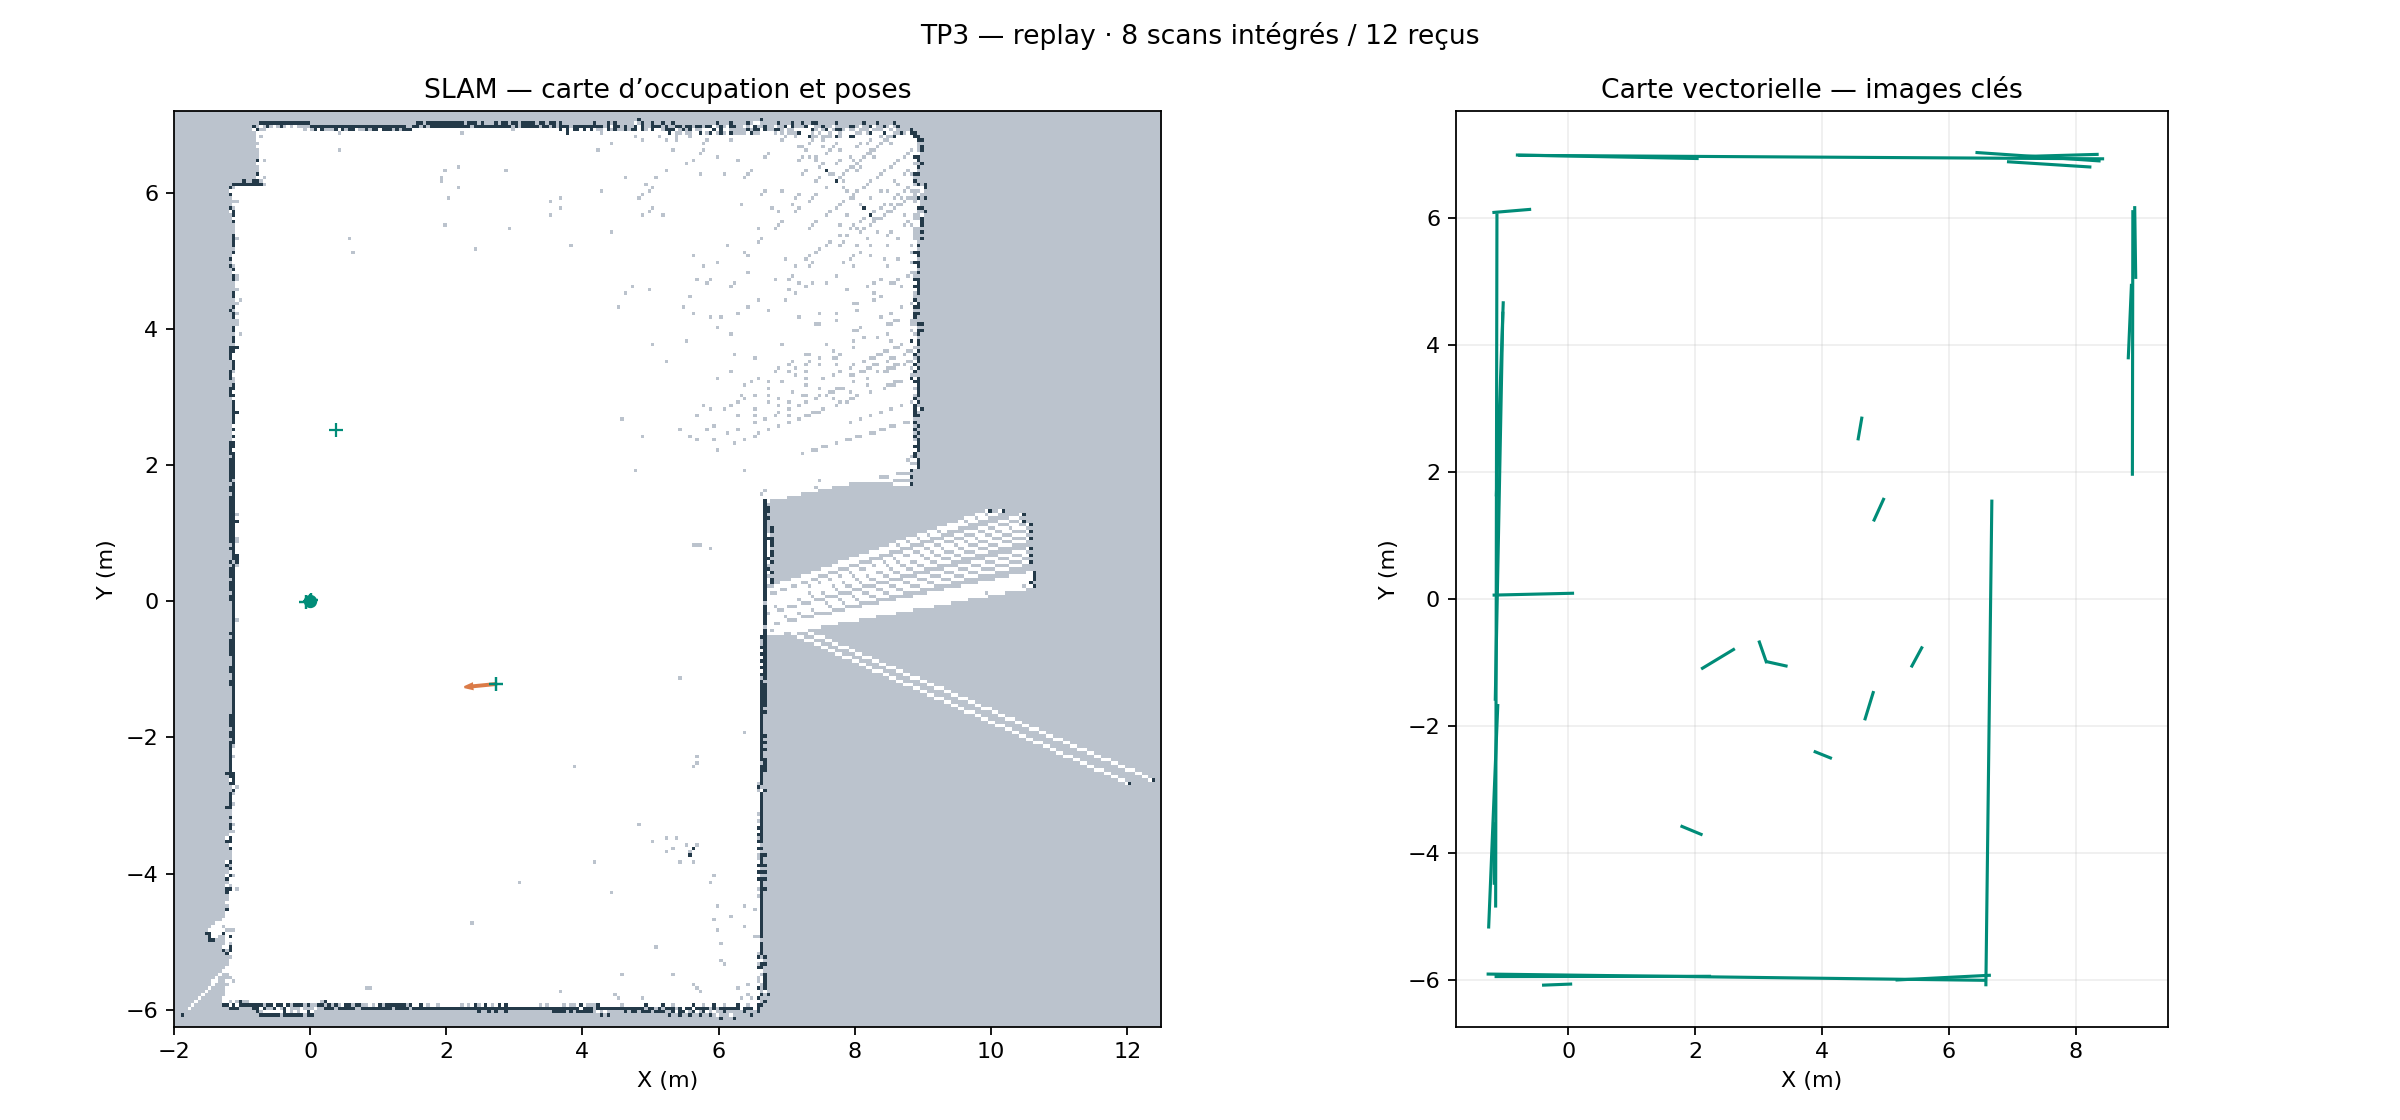
\includegraphics[width=\linewidth]{carte_salle.png}
\caption{Salle de classe reconstruite à partir des scans réels : grille
d'occupation et poses des scans intégrés (gauche), carte vectorielle
extraite des images clés (droite).}
\end{figure}

\begin{table}[htbp]
\centering
\caption{Rejeu des douze scans réels.}
\begin{tabular}{lr}
\toprule
Indicateur & Valeur \\
\midrule
Scans acceptés & 8 sur 12 \\
Images clés & 6 \\
Cellules occupées / libres & 1\,048 / 45\,082 \\
Segments de la carte vectorielle & 29 \\
Temps moyen par scan & 39 ms \\
\bottomrule
\end{tabular}
\end{table}

Les quatre scans rejetés ne satisfont pas les seuils de recalage ; ils ne
sont pas forcés dans la carte. La carte couvre la salle, mais il ne s'agit
pas d'une couverture complète vérifiée : les zones masquées par les
personnes, tables ou armoires restent inconnues. Les positions physiques
n'ayant pas été mesurées, aucune erreur de pose réelle n'est donnée.

\section{Évaluation en simulation}
Le mode simulation lance une exploration dans une scène asymétrique de
$10\times8$ m. Le robot simulé choisit des frontières entre espace libre et
inconnu, s'oriente puis avance par petits pas, en utilisant seulement les
scans et la carte construite. La scène vraie sert exclusivement à simuler
les impacts, empêcher les collisions et calculer les erreurs. Le SLAM reçoit
une prédiction de mouvement volontairement biaisée (+3\,\% en translation,
$-3$\,\% en rotation), pas la pose vraie.

\begin{figure}[htbp]
\centering
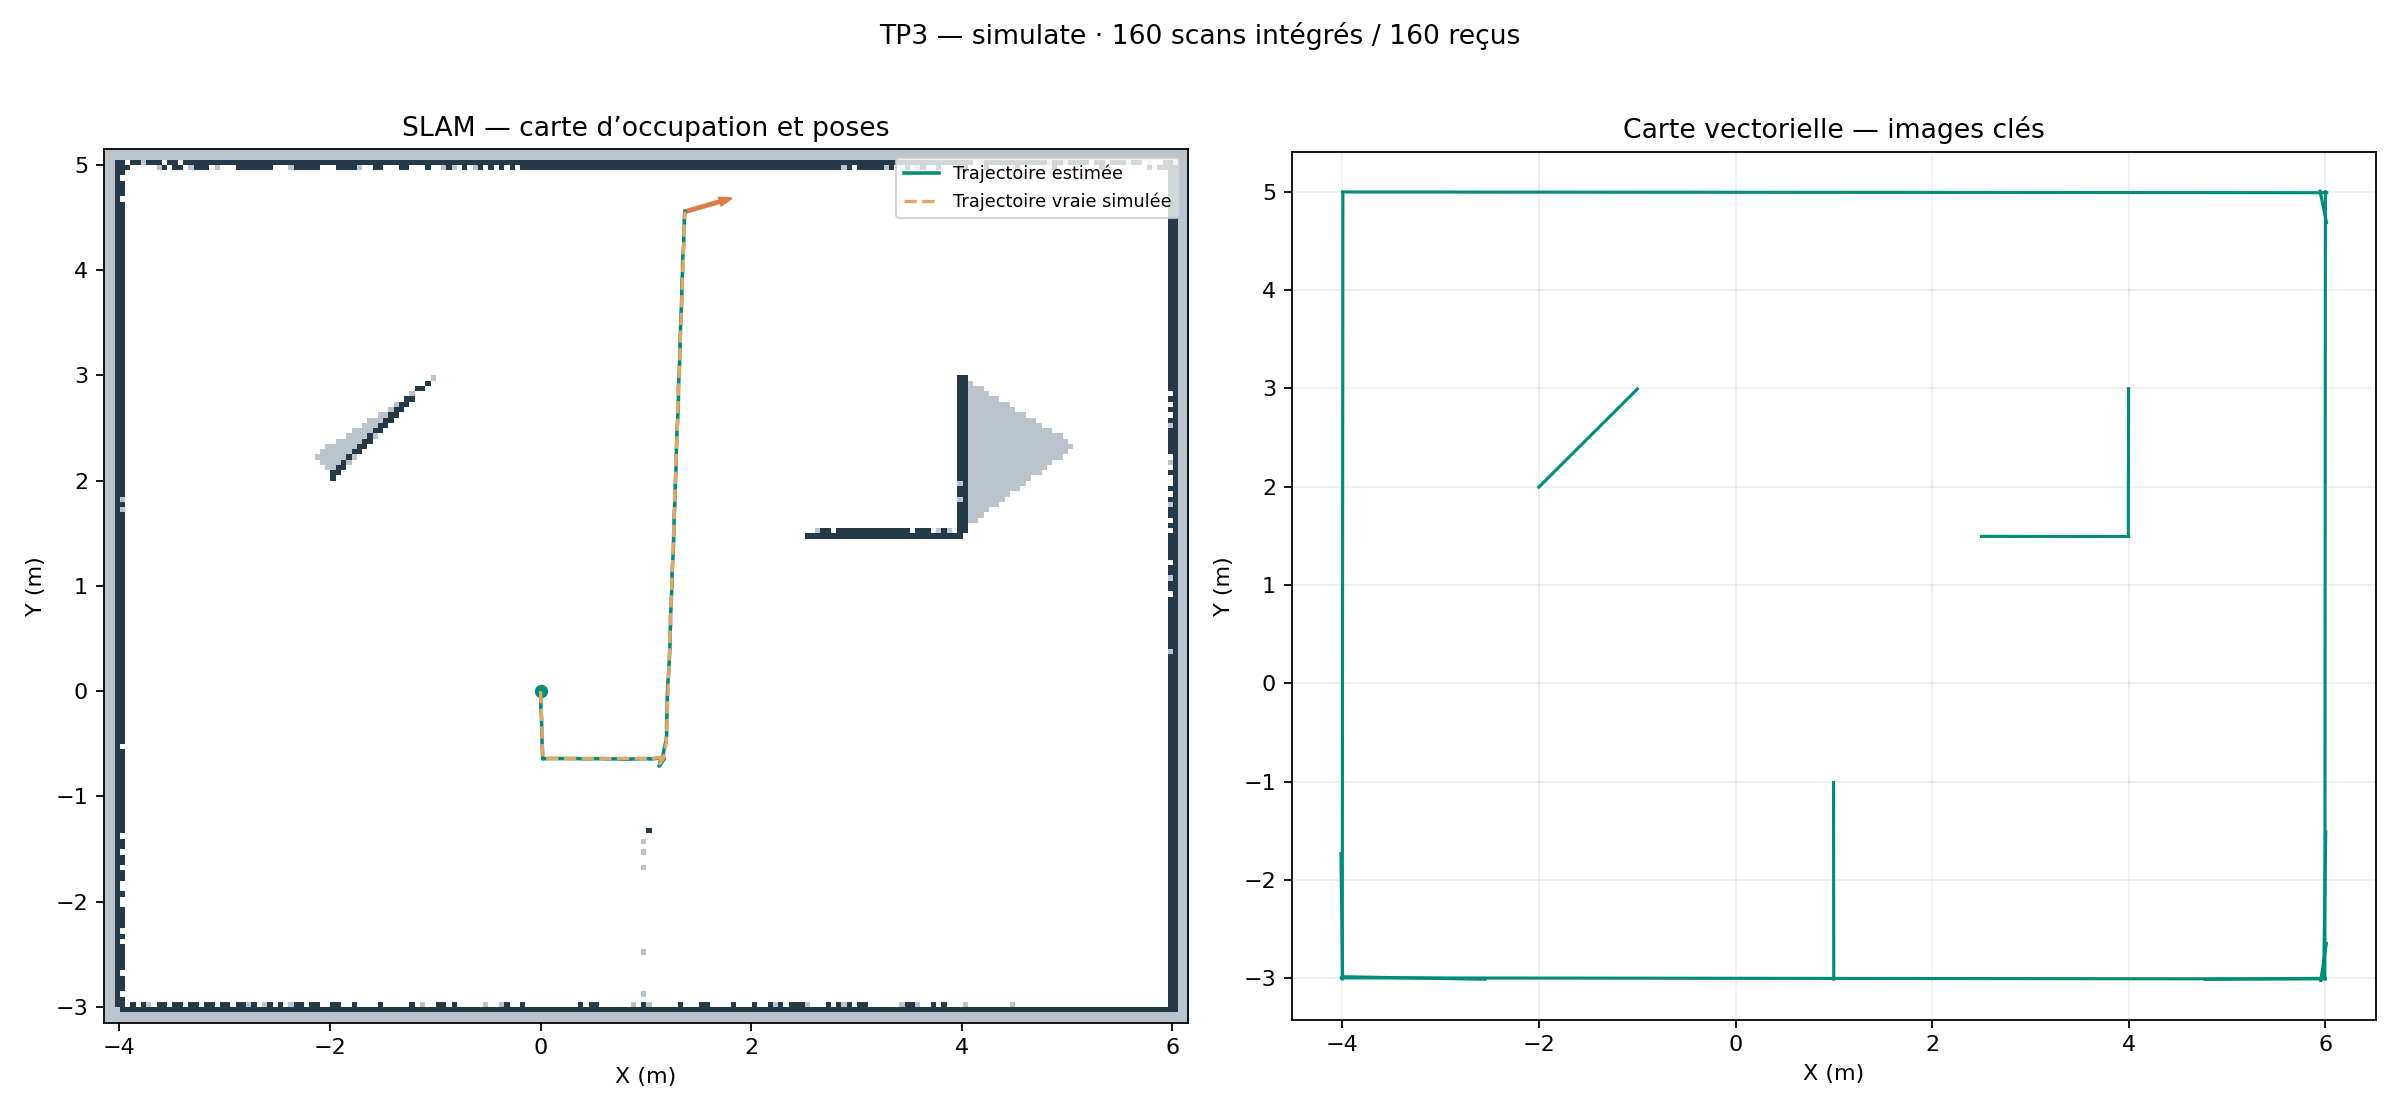
\includegraphics[width=\linewidth]{simulation.png}
\caption{Simulation de 160 acquisitions : trajectoire vraie (orange) et
estimée (vert), grille d'occupation et carte vectorielle.}
\end{figure}

\begin{table}[htbp]
\centering
\caption{Simulation de 160 acquisitions (poses vraies connues, bruit radial
de 5 mm).}
\begin{tabular}{lr}
\toprule
Indicateur & Valeur \\
\midrule
Scans intégrés & 160 sur 160 \\
Erreur de position moyenne / maximale & 0,49 cm / 1,31 cm \\
Erreur angulaire moyenne / maximale & $0,095^\circ$ / $0,24^\circ$ \\
Taux de réussite (15 cm, $2^\circ$) & 100\,\% \\
Murs retrouvés à 15 cm près & 96,4\,\% \\
Temps moyen par scan & 41 ms \\
\bottomrule
\end{tabular}
\end{table}

Aucune fermeture de boucle n'a été ajoutée pendant cette exploration ; le
retour fermé et l'optimisation du graphe sont vérifiés séparément par les
tests. Ces valeurs concernent la simulation, avec un biais d'odométrie fixe.

\section{Fonctionnement en direct}
\subsection{USB}
En mode \code{serial}, le programme lit les scans CSV envoyés par l'ESP32
et met à jour la carte en direct, sans commander de moteur. Lors de l'essai
du 4 novembre, le port USB était détecté mais aucun scan CSV complet n'a été
reçu dans le délai de 15 s : l'acquisition réelle en direct reste à valider
(alimentation du LiDAR, programme actif, sortie CSV).

\subsection{Robot en Wi-Fi}
Le sketch \code{arduino/Robot_SLAM_WiFi/Robot_SLAM_WiFi.ino} conserve les
commandes de RobotControl et ajoute la route \code{/scan_slam}, qui fournit
un numéro de scan et des horodatages : une réponse identique ou trop ancienne
n'est pas utilisée comme nouvelle observation. La boucle effectue : scan
frais, localisation, mise à jour, choix d'un trajet libre, impulsion moteur
d'au plus 0,25 s, arrêt, attente de 0,30 s, scan suivant. Le mouvement
automatique exige l'option \code{--auto} et des vitesses calibrées ; un scan
rejeté, une perte de communication ou un obstacle sans dégagement entraîne
l'arrêt. La compilation du firmware est vérifiée ; le déplacement réel ne
l'est pas.

\section{Tests}
Les tests couvrent les transformations SE(2), le rejet sans pollution de la
carte, les ambiguïtés d'orientation, le graphe ancré, la fermeture de boucle,
le maintien des petits impacts dans la grille, l'exploration, la fraîcheur
des scans et l'arrêt sur erreur réseau. Les transports réseau sont remplacés
par des doubles de test : aucun test n'envoie de commande à un robot réel.
La suite complète du dépôt compte 88 tests réussis.

\section{Comparaison avec la version améliorée}
Le dossier \code{upgrade code with IA} du dépôt contient une version
améliorée de ce SLAM, évaluée sur un banc commun plus exigeant : odométrie à
bruit aléatoire (et non un biais fixe), trajets imposés identiques pour les
deux versions, trois graines.

\begin{table}[htbp]
\centering
\caption{Banc commun, salle de classe simulée : cette version et la version
améliorée.}
\begin{tabular}{lrr}
\toprule
Indicateur & Cette version & Version améliorée \\
\midrule
Erreur moyenne de position & 15,3 cm & 5,3 cm \\
Erreur moyenne d'angle & $2,22^\circ$ & $0,47^\circ$ \\
Cellules occupées sur un vrai mur & 75\,\% & 96\,\% \\
Surface couverte en exploration & 76\,\% & 99\,\% \\
\bottomrule
\end{tabular}
\end{table}

Sur ce banc, les erreurs de cette version sont plus élevées que dans sa
propre simulation, car l'odométrie y est bruitée de façon aléatoire. Le
rapport de la version améliorée détaille les défauts mesurés et leurs
corrections.

\section{Limites}
\begin{itemize}
\item Aucune pose physique n'a été mesurée : sur les données réelles, aucune
précision métrique n'est affirmée.
\item Les douze scans ne forment pas une séquence continue ; quatre sont
rejetés avec les seuils actuels, qui ne doivent pas être abaissés pour tout
accepter.
\item Une pièce symétrique peut fournir plusieurs solutions de recalage
presque équivalentes : le programme rejette alors le scan.
\item L'acquisition en direct et le déplacement automatique n'ont pas été
validés sur le robot.
\end{itemize}

\section*{Conclusion}
\addcontentsline{toc}{section}{Conclusion}
Les outils des TP n° 1 et n° 2 sont réunis dans un SLAM incrémental qui
localise chaque scan avant de l'intégrer, corrige la dérive par un graphe de
poses et produit à la fois une grille d'occupation et une carte vectorielle.
La carte de la salle de classe est reconstruite à partir de huit des douze
scans réels. En simulation, l'erreur moyenne est de 0,5 cm et $0{,}1^\circ$.
L'étape suivante est l'essai sur le robot : acquisition continue à petits pas,
retour vers une zone déjà observée pour tester une fermeture de boucle réelle,
et calibration des vitesses avant le déplacement automatique.

\clearpage
\appendix
\section{Reproduction}
\begin{lstlisting}
python -m pip install -r requirements.txt
python -m pytest tests/test_slam.py tests/test_slam_robot.py -q

# Poses du TP 1 servant d'initialisation
D="upgrade code with IA/donnees/scans"
python merge_scans.py "$D"/*.csv \
  --reference "$D/scan_20261102_170438_115290.csv" --output resultats

# Carte de la salle
python slam_tp3.py --mode replay "$D"/*.csv \
  --anchor "$D/scan_20261102_170438_115290.csv" \
  --initial-poses resultats/poses_estimees.json --output slam/salle

# Simulation
python slam_tp3.py --mode simulate --steps 160 --output slam/simulation
\end{lstlisting}
Le guide \code{JOUR3_SLAM.md} détaille aussi les modes USB et Wi-Fi.

\end{document}
